% ----------------------------------------------------------
\chapter{Solução do modelo mecânico}
% ----------------------------------------------------------
A solução do modelo mecânico será feita através do \textit{software} ANSYS e a primeira parte desse capítulo descreverá a solução numérica pelo método dos elementos finitos (de forma mais genérica possível) comentando as opções do ANSYS, quando pertinente. Posteriormente, será dada ênfase na solução numérica envolvendo as do modelo constitutivo do material (que é o foco principal do trabalho). 

\section{Forma fraca das equações de campo}
No contexto da evolução quase estática e da hipótese das pequenas perturbações podem-se escrever as equações de campo na sua forma fraca através do princípio dos trabalhos virtuais. Sendo assim, aplicando um campo de deslocamento virtual $\dul$, cinematicamente admissível, em (\ref{eq:equilibrio_estatico_local}), porém ao longo de todo o volume $\Omega$ tem-se que:
\begin{equation}
	\label{eq:deslocamento_virtual}
	\int_{\Omega} \left(\divl \sigmall + \rho \fl \right)d\Omega \cdot \dul = 0,
\end{equation}
\begin{equation}
	\label{eq:deslocamento_virtual_2}
	\int_{\Omega} \divl \sigmall d\Omega \cdot \dul + \int_{\Omega} \rho \fl d\Omega \cdot \dul = 0.
\end{equation}

Aplicando o Teorema da Divergência no termo mais à esquerda da igualdade (\ref{eq:deslocamento_virtual_2}) obtém-se:
\begin{equation}
	\label{eq:deslocamento_virtual_3}
	\int_{\Omega} \sigmall : \dvarepsilonll d\Omega - \left(\int_{\Omega} \rho \fl \cdot \dul d\Omega + \int_{\partial \Omega} \Tl^d \cdot \dul dS \right) = U_{int} - W_{ext} = 0
\end{equation}

A expressão (\ref{eq:deslocamento_virtual}) é uma equação integral em que, no equilíbrio, o trabalho virtual das forças externas $W_{ext}$ sobre o sistema é totalmente convertido em energia potencial interna $U_{int}$  de deformação.

\section{Notação de Voigt}
Os tensores simétricos de segunda e quarta ordem são comumente representados, respectivamente, por arranjos (\textit{arrays}) vetoriais e matriciais convenientes à álgebra computacional. Dessa forma é utilizada a seguinte notação \cite[p. 682]{Zienkiewicz2005}:
\begin{equation}
	\label{eq:sigmal}
	\sigmall \rightarrow \sigmal = \left\{\sigma_{11}~~~\sigma_{22}~~~\sigma_{33}~~~\sigma_{21}~~~\sigma_{23}~~~\sigma_{31} \right\}^T
\end{equation}
\begin{equation}
	\label{eq:varepsilonl}
	\varepsilonll \rightarrow \varepsilonl = \left\{\varepsilon_{11}~~~\varepsilon_{22}~~~\varepsilon_{33}~~~2\varepsilon_{21}~~~2\varepsilon_{23}~~~2\varepsilon_{31} \right\}^T
\end{equation}
\begin{equation}
	\label{eq:Dl}
	\Dllll \rightarrow \Dll = 
	\begin{bmatrix}
		D_{1111} & D_{1122} & D_{1133}  & D_{1121} & D_{1123} & D_{1131} \\
				& D_{2222}  & D_{2233}  & D_{2221} & D_{2223} & D_{2231}  \\
				& 			& D_{3333}  & D_{3321} & D_{3323} & D_{3331}  \\
				& 			&		    & D_{2121} & D_{2123} & D_{2131}  \\
				& \text{SIM}&		    & 	       & D_{2323} & D_{2331}  \\
				& 			&		    & 	       &          & D_{3131} 
	\end{bmatrix}
\end{equation}
\begin{equation}
	\label{eq:dgdsl}
	\dgdsll \rightarrow \dgdsl = \left\{\dfrac{\partial g}{\partial \sigma_{11}}~~~\dfrac{\partial g}{\partial \sigma_{22}}~~~\dfrac{\partial g}{\partial \sigma_{33}}~~~\dfrac{\partial g}{\partial \sigma_{21}}~~~\dfrac{\partial g}{\partial \sigma_{23}}~~~\dfrac{\partial g}{\partial \sigma_{31}} \right\}^T
\end{equation}
\begin{equation}
	\label{eq:Uml}
	\Umll \rightarrow \Uml = \left\{1~~~1~~~1~~~0~~~0~~~0 \right\}^T
\end{equation}
\begin{equation}
	\label{eq:UmllotimesUll}
	\Umllll \rightarrow \Umll = 
	\begin{bmatrix}
		1 & 0 & 0 & 0 & 0 & 0 \\
		0 & 1 & 0 & 0 & 0 & 0  \\
		0 & 0 & 1 & 0 & 0 & 0  \\
		0 & 0 & 0 & 1/2 & 0 & 0  \\
		0 & 0 & 0 & 0 & 1/2 & 0  \\
		0 & 0 & 0 & 0 & 0 & 1/2 
	\end{bmatrix}
\end{equation}
\begin{equation}
	\label{eq:UmllotimesUll}
	\Umll \otimes \Umll \rightarrow  
	\begin{bmatrix}
		1 & 1 & 1 & 0 & 0 & 0 \\
		1 & 1 & 1 & 0 & 0 & 0  \\
		1 & 1 & 1 & 0 & 0 & 0  \\
		0 & 0 & 0 & 0 & 0 & 0  \\
		0 & 0 & 0 & 0 & 0 & 0  \\
		0 & 0 & 0 & 0 & 0 & 0 
	\end{bmatrix}
\end{equation}
sendo o subscrito $T$ a operação de transposição. Como se pode ver é utilizada a mesma simbologia de tensores de primeira ordem e de segunda ordem representando vetores (arranjos unidimensionais) e matrizes (arranjos bidimensionais), respectivamente. Nessa notação, as operações também são transformadas, de tal forma que:
\begin{equation}
	\label{eq:operacoes_voigt}
	\begin{array}{lcl}
		\underline{a} \cdot \underline{b} \rightarrow \underline{b}^T \underline{a}, \\ 
		\underline{\underline{a}} : \underline{\underline{b}} \rightarrow \underline{a}^T \underline{b}, \\ 
		\underline{\underline a} \otimes \underline{\underline b} \rightarrow \underline a ~ \underline b ^T, \\ 
		\underline{\underline{\underline{\underline{C}}}} : \underline{\underline{b}} \rightarrow \underline{\underline C} ~ \underline b, \\ 
		\underline{\underline{b}}:\underline{\underline{\underline{\underline{C}}}} : \underline{\underline{b}} \rightarrow \underline {b}^T \underline{\underline{C}} ~ \underline{b}, \\ 
		\left( 	\underline{\underline{\underline{\underline{C}}}}:\underline{\underline{a}} \right) \otimes \left( \underline{\underline{b}} :	\underline{\underline{\underline{\underline{C}}}} \right) \rightarrow \underline{\underline{C}}~ \underline{a}~\underline{b}^T \underline{\underline{C}}.
	\end{array}
\end{equation}

Além disso, na notação de Voigt, é necessário definir o produto termo-a-termo entre \textit{arrays} unidimensionais, de tal forma que:
\begin{equation}
	\label{eq:ab}
	\underline a ~ \underline b  = \underline c ~ \text{em que}~\underline c  = \left\{a_1b_1~~~a_2b_2~~~a_3b_3~~~a_4b_4~~~...~~~a_nb_n \right\}.
\end{equation}

Essa será a notação adotada para o restante do trabalho. Logo, o teorema dos trabalhos virtuais (\ref{eq:deslocamento_virtual_3}) pode ser reescrito da seguinte forma:
\begin{equation}
	\label{eq:deslocamento_virtual_3}
	\int_{\Omega} \dvarepsilonl^T \sigmal d\Omega - \left(\int_{\Omega} \rho \dul^T \fl d\Omega + \int_{\partial \Omega} \dul^T \Tl^d dS \right) = U_{int} - W_{ext} = 0
\end{equation}
\section{Discretização espacial em elementos finitos}
A solução por elementos finitos consiste em discretizar o domínio $\Omega$ em um conjunto de elementos contíguos $\Omega_e$, estabelecendo o que se chama de malha de elementos finitos (\autoref{discretizacao_MEF}). Cada elemento da malha tem um formato simples: linha, triângulo ou quadrilátero, tetraedro ou hexaedro, dependendo da dimensão (1D, 2D ou 3D) do domínio a ser discretizado. Cada elemento está conectado a outros elementos compartilhando "nós" sendo que a principal incógnita do problema são os deslocamentos nodais.
\begin{figure}[H]
	\begin{center}
		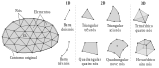
\includegraphics[scale = 1.0]{0601-discretizacao_dominio.pdf}
	\end{center}
	\caption{\label{discretizacao_MEF}Discretização de um domínio genérico em elementos finitos (adaptado de: \citeonline[p. 1-2]{DeSouza2003})}
\end{figure}

Nesse método, o campo de deslocamentos no interior dos elementos é relacionado com os deslocamentos nodais através de funções de interpolação, por exemplo, lineares ou quadráticas, cujos coeficientes são postos em função dos deslocamentos nodais. Dessa forma, o campo de deslocamentos no interior do elemento pode ser descrito como:
\begin{equation}
	\label{eq:campo_deslocamentos}
	\ul(\xl) = \ul(x_1,x_2,x_3) = \Nll(\xl)\ul_e.
\end{equation}
sendo $\ul(\xl)$ o campo de deslocamentos no interior do elemento, $\ul_e$ os deslocamentos nodais e $\Nll$ a matriz contendo as funções de interpolação (também conhecidas como funções de forma). A matriz $\Nll$  tem a seguinte estrutura:
\begin{equation}
	\label{eq:matriz_N}
	\Nll = 	\begin{bmatrix}
		N_1 & 0 & 0 & N_2 & 0 & 0 &  	& N_{n_e} & 0 & 0 \\
		0 & N_1 & 0 & 0 & N_2 & 0 & ... & 0 & N_{n_e} & 0  \\
		0 & 0 & N_1 & 0 & 0 & N_2 &  	& 0 & 0 & N_{n_e} 
	\end{bmatrix}_{n_d \times (n_e \cdot n_d)}
\end{equation}
em que $N_i$ são as funções de interpolação de cada nó $i$, $n_e$ número de nós do elemento e $n_d$ o número de dimensões. Introduzindo (\ref{eq:campo_deslocamentos}) nas equações de compatibilidade (\ref{eq:green_lagrange_linearizado}) tem-se:
\begin{equation}
	\label{eq:deformacoes}
	\varepsilonl(\xl) = \varepsilonl(x_1,x_2,x_3) = \nabla^s\ul(\xl) = \nabla^s \Nll~\ul_e = \Bll~\ul_e
\end{equation}
sendo $\varepsilonl$ o campo de deformações e $\Bll = \nabla^s \Nll$ a matriz que relaciona os deslocamentos nodais com as deformações no interior do elemento. Para problemas tridimensionais, o operador gradiente simétrico, na notação de Voigt, é dado por:
\begin{equation}
	\label{eq:gradiente_simetrico}
	\Nll = 	\begin{bmatrix}
		\dfrac{\partial}{\partial x_1} & 0 & 0  \\
		0 & \dfrac{\partial}{\partial x_2} & 0  \\
		0 & 0 & \dfrac{\partial}{\partial x_3} \\
		\dfrac{\partial}{\partial x_2} & \dfrac{\partial}{\partial x_1} & 0 \\
		0 & \dfrac{\partial}{\partial x_3} & \dfrac{\partial}{\partial x_2} \\
		\dfrac{\partial}{\partial x_3} & 0 & \dfrac{\partial}{\partial x_1}		
	\end{bmatrix}_{n_c \times n_d}
\end{equation}
em que $n_c$  é o número de componentes de deformações. Introduzindo (\ref{eq:deformacoes}) na lei de comportamento do material, é possível determinar as tensões no interior do elemento também em função dos deslocamentos nodais:
\begin{equation}
	\label{eq:tensoes}
	\sigmal(\xl) = \sigmal(x_1,x_2,x_3) = \Dll ~ \Bll ~\ul_e + \Dll ~\varepsilonl_0 + \sigmal_0
\end{equation}
na qual $\varepsilonl_0$ e $\sigmal_0$ são deformações e tensões iniciais no interior do elemento, respectivamente. Nos problemas de túneis, é através de $\sigmal_0$ que é introduzido as tensões \textit{in situ}. Para o caso de tensão geostática hidrostática, em um túnel de profundidade $H$ em um maciço com peso específico $\gamma_m$ a seguinte expressão é utilizada:
\begin{equation}
	\label{eq:tensoes_iniciais}
	\sigmal_0 = \gamma_m H \Uml
\end{equation}

Introduzindo as expressões (\ref{eq:campo_deslocamentos}), (\ref{eq:deformacoes}) e (\ref{eq:tensoes}) no princípio dos trabalhos virtuais (\ref{eq:deslocamento_virtual_3}), considerando o domínio de um elemento $\Omega_e$, obtém-se a seguinte equação de equilíbrio em forças:
\begin{equation}
	\label{eq:forcas_interna_externa}
	\Fl_{int_e} - \Fl_{ext_e} = \underline 0
\end{equation}
em que:
\begin{equation}
	\label{eq:forca_interna}
	\Fl_{int_e} = \int_{\Omega_e} \Bll^T \sigmal d\Omega_e = \Kll_e \ul_e + \Fl_{\varepsilon_{0_e}} + \Fl_{\sigma_{0_e}}
\end{equation}
\begin{equation}
	\label{eq:forca_externa}
	\Fl_{ext_e} = \Fl_{V_e} + \Fl_{S_e} + \Fl_{C_e} + \Fl_{N_e}
\end{equation}
nos quais:
\begin{equation}
	\label{eq:elementos_forca_interna}
	\Kll_e = \int_{\Omega_e} \Bll^T \sigmal d\Omega_e,~~~ \Fl_{\varepsilon_{0_e}} = \int_{\Omega_e} \Bll^T \Dll~ \varepsilonl_0 d\Omega_e,~~~ \Fl_{\sigma_{0_e}} = \int_{\Omega_e} \Bll^T \sigma_0 d\Omega_e,
\end{equation}
\begin{equation}
	\label{eq:elementos_forca_externa}
	\Fl_{V_e} = \int_{\Omega_e} \rho \Nll^T \fl d\Omega_e,~~~ \Fl_{S_e} = \int_{\partial \Omega_e} \Nll^T \Tl^d dS_e,~~~
	\Fl_{C_e} = \int_{\partial \Omega_{e}} \Nll^T \Tl^c dS_c,
\end{equation}
sendo que $\Fl_{int_e}$ e $\Fl_{ext_e}$ são as forças internas e externas no elemento, respectivamente, $\Kll_e$ a matriz de rigidez do elemento, $\Fl_{\varepsilon_{0_e}}$ e $\Fl_{\sigma_{0_e}}$  forças internas no elemento devido às deformações inciais e tensões iniciais, respectivamente, $\Fl_{V_e}$ forças de volume do elemento, $\Fl_{S_e}$ forças de superfície no contorno livre do elemento, $\Fl_{C_e}$ forças de contato entre elementos vizinhos e $F_{N_e}$  forças nodais. A Figura 6.2 ilustra as forças externas de um elemento genérico.
\begin{figure}[H]
	\begin{center}
		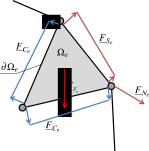
\includegraphics[scale = 1.0]{0602-diagrama de corpo livro de um elemento finito.pdf}
	\end{center}
	\caption{\label{discretizacao_MEF}Diagrama de corpo livre de um elemento finito (adaptado de: \citeonline[p. 19]{Lizarza2011})}
\end{figure}
No método dos elementos finitos, as integrais de volume no domínio  $\Omega_e$, por eficiência, são geralmente resolvidas em um domínio de referência $\Omega_\xi$ com geometria normalizada $-1 \le \xi_i \le 1$. As coordenadas $\underline \xi$ também são conhecidas como coordenadas naturais do elemento. Portanto, é feita a seguinte troca de variáveis nas integrais de volume (DHATT et al. 2012):



\section{Solução do sistema e discretização temporal}

\section{Algoritmo de atualização das tensões e variáveis internas}

\subsection{Integração das equações constitutivas elastoplásticas}


\subsubsection{Esquema de integração totalmente implícito}


\subsubsection{Esquema de integração semi-implícito}


\subsection{Atualização do módulo constitutivo}

\subsection{Particularizando para estado plano de deformações e axissimetria}

\subsection{Domínios, discretização, condições de contorno e ciclo construtivo para os modelos de verificação}


